\documentclass{report}

\usepackage[a4paper, total={6in, 8in}, margin=1in,footskip=0.25in]{geometry}
\usepackage{amsmath, amsthm, amssymb, booktabs, chemfig, graphicx, float, pgfplots, upgreek, siunitx, multirow, multicol}
\usepackage[hidelinks]{hyperref}

\usepackage{chemmacros}
\chemsetup[phases]{pos=sub}
\chemsetup[reactants]{concentration-unit=\moLar}
\chemsetup{
  formula = mhchem, % or mhchem
}

\DeclareSIUnit{\solub}{\unit[per-mode=symbol]{\gram\per\qty{100}{\gram}\,\ce{H2O}}}

\setlength{\parindent}{0pt}
\setlength{\parskip}{0.8em}

\pgfplotsset{compat=1.18}

\graphicspath{{../../Images/}}

\title{\Huge Year 12 Chemistry}
\author{L. Cheung}

\begin{document}
\maketitle
\tableofcontents
\DeclareSIUnit{\molar}{\mole\per\liter}


% !TEX root = ./chemistry.tex

\chapter{Module 5 \; Equilibrium and Acid Reactions}

\section{Le Chatelier's Principle} \label{29/10/2024-31/10/2024}
	"If a system at equilibrium is subject to a change in conditions, then the system will behave in such a way so as to partially counteract the imposed change"

	Haber process:

	\subsection{Effect of Concentration}
		\begin{equation}
			\ce{N2\gas{} + 3H2\gas{} <=> 2NH3\gas{} \quad \enthalpy{-92.5}}
		\end{equation}
		

	\subsection{Effect of Pressure}
	\subsection{Effect of Partial Pressure}
	\subsection{Effect of Volume}
		Decreasing the volume will increase the pressure. (Boyle's Law) This increases the collision rate between the reactants and favours the forward reaction.

	\subsection{Effect of Temperature}
		filler text
	
	\subsection{Summary}
		To use Le Chatelier's principle to predict the outcome of a change in conditions, you need to consider the following points.
		\begin{enumerate}
			\item What change is imposed?
			\item What is the opposite of the change?
			\item Which reaction direction is favoured - the forward or reverse?
			\item Does equilibrium shift to the left or right?
			\item What happens to the concentrations of each aqueous substance or gas?
		\end{enumerate}

	\begin{figure}[H]
		\centering
		\includegraphics{Le Chatelier's example problem}
	\end{figure}

	\textbf{D} When temperature decreases, the rates of both forward and backward reactions will decrease regardless of which way the endothermic or exothermic reaction goes. (A and B can be eliminated)

	This is because all the particles in the system lose kinetic energy, decreasing the rate of collisions hence, decreasing the rate of reaction.
	
	However, since there is a decrease in temperature the exothermic reaction will be favoured in order to counteract the change. In this case, the forward reaction being exothermic is affected less by the drop in temperature as shown in D.

\pagebreak
\section{Practical Investigation 2.3 - Effect of changes to concentration on equilibrium} \label{31/10/2024}

	Aim: To observe the effect of a change in concentration on a system at equilibrium

	\subsection{Materials}
		\begin{itemize}
			\item 2 mL of 0.1 molL$^{-1}$ iron(III) chloride solution
			\item 2 mL of 0.1 molL$^{-1}$ ammonium thiocyanate solution
			\item 1 mL of 0.1 molL$^{-1}$ calcium fluoride solution
			\item 20 mL distilled water
			\item 2x 10 mL measuring cylinders
			\item 25 mL measuring cylinder
			\item 4 test tubes
			\item Test-tube rack
			\item 4 small labels
			\item Disposable 1 mL droppers
			\item Waste bottle
			\item Digital camera
			\item Safety glasses
		\end{itemize}

	\subsection{Risk Assessment}
		\begin{table}[htbp]
			\centering
			\begin{tabular}{l|l}
				\hline
				Hazard & Precaution \\ \hline
				Chemicals may splash onto skin or eyes & Wear safety glasses and wash hands  \\
				Chemicals may harm aquatic life & Place in inorganic waste container \\
			\end{tabular}
		\end{table}

	\subsection{Method}
		\begin{enumerate}
			\item Pour 1 mL of iron(III) chloride solution into a 10 mL measuring cylinder.
			\item Pour 1 mL of ammonium thiocyanate into another 10 mL measuring cylinder.
			\item Pour both solutions into the 25 mL measuring cylinder.
			\item Add 18 mL of distilled water to the 25 mL measuring cylinder so that the total volume is 20 mL.
			\item Label four test tubes A, B, C and D.
			\item Pour equal volumes of the solution in the 25 mL measuring cylinder into each of the test tubes.
			\item Retain test tube A as the reference solution.
			\item Add 1 mL of iron(III) chloride to test tube B.
			\item Take a photo to record observations for test tube B relative to test tube A.
			\item Add 1 mL of ammonium thiocyanate to test tube C.
			\item Take a photo to record observations for test tube C relative to test tube A.
			\item Add 1 mL of calcium fluoride to test tube D. (Note: This reacts with the iron(III) ion so there is less iron(III) available to react with the thiocyanate ion.)
			\item Take a photo to record observations for test tube D relative to test tube A
		\end{enumerate}

	\subsection{Results}
		\begin{figure}[H]
			\centering
			\includegraphics{Practical Investigation 2.3 - Results.png}
			\caption{Test tubes A, B, C, D}
		\end{figure}

	\subsection{Discussion}
		\textbf{Explain each colour change in terms of collision theory.}

		The test tube B was darker in colour in comparison to test tube A. The increase in moles of reactants allows more successful collisions to occur, increasing the amount of product. The same principle applies to test tube C.

		Test tube D was lighter in colour compared to A, due to the calcium fluoride reacting with the iron (III) chloride 

	\subsection{Conclusion}
		\textbf{Use Le Chatelier's principle to explain what happened in test tubes B, C and D.}

		Test tube B was darker due to the increase in concentration of the reactant iron (III) chloride causes a shift of the equilibrium towards the products due Le Chatelier's principle
		
		Test tube C was darker due to the increase in concentration of the reactant ammonium thiocyanate causes a shift of the equilibrium towards the products due Le Chatelier's principle

		Test tube D was lighter because the calcium fluoride reacted with the iron (III) chloride, lowering the overall concentration of iron (III) chloride. This reduced the amount of reactants available, making the reverse reaction more favourable by Le Chatelier's principle.

\section{Calculating the Equilibrium Constant} \label{5/11/2024}
	The equilibrium constant can be used to predict the direction of chemical reactions

	$$K_{eq} = \frac{[products]}{[reactants]}$$
	For reaction:
	$$\ce{aA + bB <=> cC + dD}$$
	the equilibrium expression is:
	$$K_{eq}=\frac{[C]^{c}[D]^{d}}{[A]^a[B]^b}$$

	The concentration of each chemical species is raised to the power of the number of moles of that species indicated in the chemical equation. (Eg. there are $d$ moles of species $D$, hence in the equilibrium expression the concentration of species $D$ is raised to the power of $d$, written as $[D]^d$)

	\begin{itemize}
		\item The value for the equilibrium constant only takes into account the concentration of substances where the concentration can vary
		\item Solutions and gases can vary in concentration or partial pressure hence are included in $K_{eq}$
		\item Solids and pure liquids are NOT included eg. $\ce{H_2O}$ isn't required when calculating
	\end{itemize}

	\subsection{Reaction Quotient ($Q$)}
		$$Q=\frac{[C]^{c}[D]^{d}}{[A]^a[B]^b}$$
		Has the same formula as $K_{eq}$, however applies to any stage of a reaction
		
	\subsection{Equilibrium Constant}
		\begin{itemize}
			\item Comparing $Q$ to $K_{eq}$ predicts which way the equilibrium will shift
			\item $K_{eq}$ is where the equilibrium lies
			\item A large $K_{eq}$ means that there are more products than reactants; ie. equilibrium lies towards completion
			\item If $K_{eq}$ is close to one, both reactants and products are plentiful at equilibrium
		\end{itemize}
		\textbf{Example} Let $Q=2.1$, $K_{eq}=0.315$, $\therefore$ products$>$reactants.

	\subsection{Calculating the equilibrium expression}
		Consider the reaction between hydrogen and iodine producing hydrogen iodide:
		$$\ce{H_{2}\gas{} + I_{2}\gas{} <=> 2HI\gas}$$

\section{ICE Tables} \label{6/11/2024}
	\begin{table}[htbp]
		\centering
		\begin{tabular}{|l|l|l|l|}
			\hline
			 & [A] & [B] & [C] \\ \hline
			Initial concentration &  &  &  \\
			Change in concentration &  &  &  \\
			Equilibrium concentration &  &  &  \\ \hline
		\end{tabular}
	\end{table}

	$$\Delta c = c_{eq}- c_{u}$$

	Eg. $\ce{A + B <=> C + D}$

	\begin{table}[htbp]
		\centering
		\begin{tabular}{lllll}
			\hline
			 & [A] & [B] & [C] & [D]  \\ \hline
			Initial concentration 		& 0.6 & 0.6 & 0 & 0 \\
			Change in concentration 	& -0.5 & -0.5 & +0.5 & +0.5 \\
			Equilibrium concentration 	& 0.1 & 0.1 & 0.5 & 0.5 \\ \hline
		\end{tabular}
	\end{table}

	Eg. $\ce{2X \gas{} <=> 3Y \gas{} + 4Z \gas{}}$

	A sample consisting of 0.500 mol of X is placed into a system with a volume of 0.750 litres. \\
	At equilibrium, the amount of sample X is known to be 0.350 mol.

	\begin{table}[htbp]
		\centering
		\begin{tabular}{cccc}
			\hline
			 & X & Y & Z \\ \hline
			I 		& 0.5 & 0 & 0 \\
			C 		&  &  & \\
			E 		& 0.35 &  &  \\ \hline
		\end{tabular}
	\end{table}

	\begin{table}[htbp]
		\centering
		\begin{tabular}{cccc}
			\hline
			 	& X & Y & Z \\ \hline
			I 		& 0.5 & 0 & 0 \\
			C 		& -0.15 & -0.225 & +0.3 \\
			E 		& 0.35 & 0.225 & 0.3 \\ \hline
		\end{tabular}
	\end{table}

	\begin{align*}
		[X] &= \frac{0.35}{0.75} = 0.467 \\
		[Y] &= \frac{0.225}{0.75} = 0.3 \\
		[Z] &= \frac{0.3}{0.75} = 0.4
	\end{align*}
	
\section{Effect of Temperature on $K_{eq}$} \label{8/11/2024}
	Although other factors may affect equilibrium, $K_{eq}$ is only affected by temperature.
	Changing concentration, pressure, or volume will change the concentrations and therefore adjust the reaction point, however the reaction will still equalise to achieve the same $K_{eq}$

	\begin{itemize}
		\item For a particular reaction, $K_{eq}$ is constant at a given temperature
		\item Temperature changes the ratio of products and reactants, hence changing $K_{eq}$
		\item For $\ce{N2O2 \gas{} <=> 2NO2 \gas{}}$, temperature increases the $K_{eq}$ value and favours the formation of products. The forward reaction is endothermic
	\end{itemize}

	\subsection{Example Question}
		Nitric oxide gas ($\ce{NO}$) can be produced from the direct combination of nitrogen gas and oxygen gas in a reversible reaction.
		\begin{enumerate}
			\item \textbf{Write a balanced chemical equation for this reaction (1 mark)}
				\subitem $\ce{N2 \gas{} + O2 \gas{} <=> 2NO \gas{}}$
			\item \textbf{Explain, using collision theory, how an increase in temperature would affect the value for $K_{eq}$ for this system. Refer to the diagram in your answer.}
				\subitem An increase in temperature would favour the forward reaction, hence $K_{eq}$ will increase. More energy allows more collisions to occur
		\end{enumerate}
	
		\begin{align*}
			K_{eq} &= \frac{[p_1][p_2]}{[r_1][r_2]} \\
			1 &= \frac{[1][1]}{[1][1]} \\
		\end{align*}
		\text{\centering If $p_2$ decreases to $[0.5]$, favouring the forward reaction}
		\begin{align*}
			&= \frac{[1.15][0.65]}{[0.85][0.85]} \\
			&=K_{eq}
		\end{align*}

\section{Use of $K_{eq}$ for the Dissociation of Ionic Solutions} \label{12/11/2024}
	Different ionic compounds have different solubilities

	Example reaction

	$$\ce{AgNO3 \aq{} + NaCl \aq{} -> AgCl \sld{} + NaNO3 \aq}$$

	Complete ionic equation: $\ce{Ag+ + NO3-}$
	
	\section{Beer Lambert Law} \label{14/11/2024}
	\begin{align*}
		\text{Absorbance} &= \text{Molar absorbility} \times \text{Path length} \times \text{Concentration} \\
		A &= \epsilon lc
	\end{align*}
	\begin{itemize}
		\item Absorbance has a direct relationship to concentration
		\item Greater concentration, greater absorbance
	\end{itemize}
	
\section{Practical Investigation 3.2}
	Aim: To use colourimetry to determine the equilibrium constant for the reaction of iron(III) ions with thiocyanate ions to form the iron(III) thiocyanate ion

	\subsection{Materials}
		\begin{itemize}
			\item 200 mL 0.2 \unit{\moLar} $\ce{Fe(NO3)3}$
			\item 100 mL 0.002 \unit{\moLar} $\ce{KSCN}$
			\item 500 mL 0.5 \unit{\moLar} $\ce{HNO3}$
			\item 60 mL 0.002 \unit{\moLar} $\ce{Fe(NO3)3}$
			\item 150 mL distilled water
			\item 6 * 100 mL volumetric flasks
			\item 5 * 150 mL beakers
			\item 2 * 100 mL beakers
			\item 1 * 25 mL bulb pipette
			\item 2 * 10 mL graduated pipettes
			\item 1 * 10 mL bulb pipette
			\item 2 pipette bulbs
			\item 1 disposable pipette
			\item Waste bottle
			\item 14 small labels
			\item 1 colourimeter and set of cuvettes
			\item Safety glasses
		\end{itemize}

	\subsection{Risk Assessment}
		\begin{table}[htbp]
			\centering
			\begin{tabular}{ll}
				\hline
				Hazard & Precaution \\ \hline
				Breaking glassware & Keep glassware on inside of table, do not run with glassware \\
				Spillage of solutions & Handle with caution, clean any spills immediately \\
				Splashing of solution into eyes & Wear safety goggles \\ \hline
			\end{tabular}
		\end{table}
	
	\subsection{Method}
	\begin{enumerate}
		\item Label the six volumetric flasks A-F.
		\item Use a 25 mL bulb pipette to transfer 25.00 mL of the 0.200 \unit{\moLar} $\ce{Fe(NO3)}$\item 3 to flask A.
		\item Use a graduated 10 mL pipette to transfer 1.00 mL of the 0.002 \unit{\moLar} \item $\ce{KSCN}$ to flask A.
		\item Add HNO3 to make a final volume of 100.00 mL.
		\item Make solutions with known concentration by pushing equilibrium as far as possible to the products. $\ce{HNO3}$ can be used to reduce the concentration of $\ce{H3O}$
		\item Rinse the cuvette with distilled water.
		\item $\frac{3}{4}$ fill the cuvette with distilled water and wipe the clear sides. 
		\item Turn on the colourimeter and turn the light to blue or 470 nm.
		\item Use the cuvette with distilled water to calibrate the colourimeter. Note: Orientate the cuvette correctly in the colourimeter so that the light passes through the clear sides of the cuvette.
		\item Rinse, a 100 mL beaker with standard solution A - it is easier to pour the solution into the cuvette using a beaker than using a volumetric flask.
		\item Rinse, then $\frac{3}{4}$ fill the cuvette with standard solution A and measure the absorbance with the colourimeter.
		\item Repeat steps 10 and 11 for the other standard solutions (B-F)
	\end{enumerate}

\section{Solution Equilibria - Dissolution of Ionic Compounds} \label{19/11/2024}
	\subsection{Factors influencing solubility}
		\begin{itemize}
			\item Activation energy required to break lattice
				\begin{itemize}
					\item Strength of ionic bonding
					\item Size of ions
					\item Charge of ions
				\end{itemize}
			\item As temperature increases, generally solubility increases
		\end{itemize}

% !TEX root = ./chemistry.tex

\chapter{Module 6 \hspace{0.5em} Acid and Base Reactions} \label{12/12/2024}

	\section{Introduction to Acid and Bases}
	
		\textbf{General Properties of Acids}
		
			\begin{itemize}
				\item Sour taste
				\item Low pH
				\item Turn blue litmus paper red
				\item Corrosive
			\end{itemize}

		\textbf{General Properties of Bases}
			
			\begin{itemize}
				\item Bitter taste (eg. caffeine)
				\item High pH
				\item Turn red litmus paper blue
				\item Corrosive and caustic
			\end{itemize}

	\section{Indicators}
	
		Indicators are substances added to solutions to show their pH. They show the concentration of hydrogen ions in a solution through a colour change.

		Most indicators are \textbf{weak acids or bases} meaning they exist in equilibrium.acids or

		\begin{center}
			\ce{HIn <=> H+ + In-}, where \ce{In} stands for indicator
		\end{center}

		Eg. Added to an acidic solution:
		\begin{enumerate}
			\item Equilibrium is disturbed by the increase of \ce{H+} ions
			\item Equilibrium therefore shifts left to decrease this concentration (LCP)
			\item As a result, the concentration of \ce{HIn} Increases, therefore changing the colour
		\end{enumerate}

		Indicators are more useful in clear, colourless solutions that make it easier to identify the equivalence point.

		\textbf{Example Question}

			\begin{figure}[H]
				\centering
				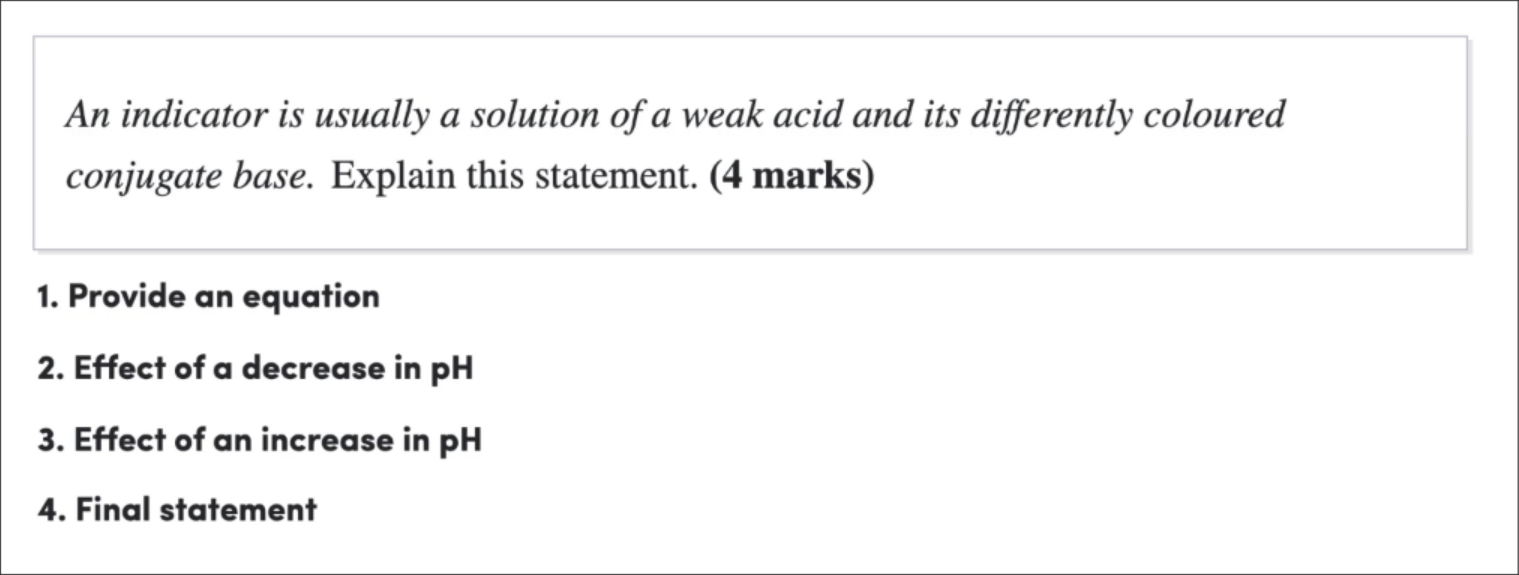
\includegraphics[width=15cm]{indicators_question.png}
			\end{figure}

		\subsection{Common Indicators}
		
			\begin{table}[H]
				\centering
				\setstretch{1.5}
				\begin{tabular}{p{4cm}| p{5cm} | p{5cm}}
					Indicator	& pH Range	& Colour (increasing pH) \\ \hline
					Methyl orange	& 3.1 - 4.4	& Red - Orange - Yellow \\
					Liquid litmus	& 4.5 - 8.3	& Red - Purple - Blue \\
					Bromothymol blue& 6.0 - 7.6	& Yellow - Green - Blue \\
					Phenolphthalein	& 8.3 - 10.0	& Colourless - Pale pink - Bright pink \\
					Universal indicator & All pH	& Red - Violet
				\end{tabular}
			\end{table}

\section{Practical Investigation 5.1 - Preparing and using natural indicators}

	Aim: To prepare and test natural indicators on a range of substances to determine their acidity or alkalinity

	\subsection{Materials}
		\begin{itemize}
			\item Plant material that acts as an indicator (Eg. red cabbage, blueberries, turmeric, petals from violets, geranium, petunias)
			\item Approx. 5mL of:
			\begin{itemize}
				\item \qty{0.1}{\moLar} NaOH
				\item \qty{0.1}{\moLar} HCl
				\item white vinegar
				\item household ammonia
				\item lemon juice
				\item lemonade
				\item bicarbonate of soda
				\item washing powder
				\item antacid tablet
				\item salt water
			\end{itemize}
			\item Distilled water
			\item \qty{500}{mL} beaker
			\item \qty{100}{mL} beakers
			\item Test tubes
			\item Test-tube rack
			\item \qty{10}{mL} measuring cylinder
			\item Knife
			\item Cutting board
			\item Mortar and pestle
			\item Kettle (for warm water)
			\item Hotplate
			\item Spatula
			\item Droppers
			\item Stirring rod
			\item Strainer or filter paper and funnel
			\item Safety glasses
		\end{itemize}

	\subsection{Risk Assessment}
		\begin{table}[H]
			\centering
			\begin{tabular}{ll}
				\hline
				Hazard & Precaution \\ \hline
				Acids are corrosive, irritate eyes & Handle with caution \\
				Bases are caustic, irritate eyes & Handle with caution \\ \hline
				Ammonia is caustic & Use in well ventilated areas \\ \hline
			\end{tabular}
		\end{table}
	
	\subsection{Method}
		\begin{enumerate}
			\item For the red cabbage: Finely shred two leaves of cabbage, place in 500 mL beaker and just cover with distilled water (about 200 mL). Slowly boil the cabbage leaves until the water turns a dark reddish-purple and the leaves lose most of their colour.
			\item Allow to cool and pour the liquid off into a clean 100 mL beaker. This is the red cabbage indicator. Note: If the colour of the solution is pale, further boiling may be necessary to concentrate the solution.
			\item For other plant material: Cut the material into small pieces and place in a mortar and pestle. Grind the material to a paste, add 5-10 mL of warm water and stir.
			\item Strain the solution into a beaker to remove any solids.
			\item Place 2 mL of each of NaOH and HCl into clean separate test tubes. Add a few drops of one indicator to each test tube until a definite colour is observed. Record the indicator and its colour in your results table.
			\item Repeat step 5 with other indicators and record your results in the table. 
			\item Repeat steps 5 and 6 with other substances. Classify the substances as acidic, basic or neutral.
			\item Place 2 mL of HCl in a clean test tube. Choose an indicator that produced a good colour difference between acid and base and add a few drops to the test tube.
			\item Add NaOH a few drops at a time to the HCl test tube until the colour no longer changes. Record any colour changes that occur during the addition of NaOH.
			\item To the test tube from step 9 add HCl a few drops at a time until the colour no longer changes. Record any colour changes.
		\end{enumerate}

	\subsection{Results}

	\subsection{Discussion}
		\begin{enumerate}
			\item \textbf{Identify which indicators would be most effective in identifying acidic, basic and neutral solutions. Provide 
			a reason for your choice.}
			Acid
			Neutral
			Basic
			\item \textbf{Which indicators, if any, were not effective in distinguishing between acidic, basic and neutral solutions? 
			Suggest possible reasons for this.}
			\subitem The beetroot and blue tea indicators were not as effective compared to the universal indicator. For unknown solutions, universal indicator allows identification of the pH. Blue tea has a lower concentration of anthocyanin compared to the beetroot solution, therefore was less effective as an indicator.
			\item \textbf{Using your results, justify whether or not indicator colour change is a reversible reaction.}
			\subitem It is a reversible reaction
		\end{enumerate}
	
	\subsection{Conclusion}
	\begin{enumerate}
		\item \textbf{Explain why indicators give a range of colours in different acid and alkaline solutions.}
	\end{enumerate}

\section{History of Acid-Base Models} \label{10/02/2025}
	\textbf{Lavoisier - Acids contain oxygen}
	\begin{itemize}
		\item Correct for some acids, eg. $\ce{H2SO4}$
		\item However doesn't apply to all acids, eg. $\ce{HCl}$ doesn't have oxygen
	\end{itemize}

	\textbf{Davy - Acids contain displaceable hydrogen}
	\begin{itemize}
		\item Considered reactions with metals and acid
		\item $\ce{H2}$ gas produced as metal displaces hydrogen in acid
		\item $\ce{H2(g) + 2HCl(aq) -> H2(g) + MgCl2(aq)}$
	\end{itemize}

	\textbf{Arrhenius - Acids ionise in water to form H+ ions}
	\begin{itemize}
		\item $\ce{HA(aq) -> H+(aq) + A-(aq)}$
		\item $\ce{XOH(aq) -> X+(aq) + OH-(aq)}$
		\item Couldn't explain why ammonia was a base
		\item Nature and role of the solvent was not considered
		\item All salts produced by reactions of an acid and base should be neutral, but acetic acid and sodium hydroxide results in a basic solution
	\end{itemize}

\section{Ammonia Dilemma} \label{12/02/2025} TODO:
	Ammonia ionises in water and produces $\ce{OH-}$ ions, and is therefore classified as an Arrhenius base. However, considering the following reaction:

	$$\ce{NH3(g) + HCl(g) -> NH4Cl(s)}$$

	The above reaction is an acid ($\ce{HCl}$) base (\ce{NH3}) reaction, however it doesn't form water.

	\subsection{Bronsted-Lowry Model}
 		Acids are proton donors, bases are proton acceptors
		\bgroup
			\centering
			\ce{HCl(aq) + H2O(l) -> H3O+(aq) + Cl-(aq)}
		\egroup

		In the above reaction, \ce{HCl} accepts a proton from \ce{H2O}, $\therefore$ \ce{HCl} = acid, \ce{H2O} = base

		\bgroup
			\centering
			\ce{NH3(aq) + H2O(l) -> NH4+(aq) + OH-(aq)}
		\egroup

		Water is \textbf{amphiprotic}, ie. can act as an acid or a base.

		\bgroup
			\centering
			\ce{2H2O <=> H3O+ + OH-}
		\egroup

		Limitations:
		\begin{itemize}
			\item Requires a solvent and doesn't explain for non-aqueous solutions
			\item Cannot explain for acidic oxides, eg. \ce{CaO(s) + SO3(g) -> CaSO4(s)}
			\item \ce{BF3}, \ce{AlCl3} act as acids, however have no \ce{H+} to donate.
		\end{itemize}

	\subsection{Lewis Model}
		Acid is an electron pair acceptor, base is an electron pair donator
		
		Explains the \ce{BF3 + NH3} reaction:

		Boron accepts a pair of electrons from the nitrogen in ammonia. Although no proton is transferred, it is still an acid-base reaction

\section{Practical Investigation 5.2 - Measuring the enthalpy of neutralisation} \label{13/02/2025}
	\textbf{Aim:} To determine the enthalpy of neutralisation and the effect of the state of the reactants

	\subsection{Materials}
		\begin{itemize}
			\item 4g NaOH
			\item 100mL 1.0 molL$^{-1}$ HCl
			\item 50mL 2.0 molL$^{-1}$ HCl
			\item 50mL 2.0 molL$^{-1}$ NaOH
			\item 100mL measuring cylinder
			\item -10-110$\degree$C thermometer or temperature probe and data logger
			\item Spatula
			\item Electronic balance
			\item 2 polystyrene cups
			\item Safety glasses
		\end{itemize}

	\subsection{Analysis of Results}
		\textbf{Part A}
		\begin{enumerate}
			\item Heat of reaction:
		\end{enumerate}
	\subsection{Discussion}

\newpage

\section{pH Scale} \label{17/02/2025}
	\begin{itemize}
		\item pH scale is a quantitative measurement of the acidity of a solution, generally between 0-14, where 7 is neutral, there are values outside the range
		\item Lower values are acids, higher values are basic
		\item Each step on the scale represents a factor of 10, ie. logarithmic scale
		\item Eg. pH 6 is 10x stronger than pH 5
		\item The term pH stands for "potential of hydrogen"
		\item The scale is based on the concentration of hydrogen ions in solution
		\item Remember that in aqueous solutions, the hydrogen ion attaches to a water molecule to form
	\end{itemize}
	The \textbf{lower} the pH, the \textbf{more acidic} a solution is
	Therefore, at 25\degree C, acids have a pH of less than 7 and bases have a pH greater than 7. A substance that has a pH equal to 7 is neutral
	pH is the concentration of $\ce{H+}$
	$$pH = -log_{10}{[\ce{H+}]}$$
	$$pOH = -log_{10}{[\ce{OH-}]}$$
	
	\subsection{Why is pH important?}
		\begin{itemize}
			\item Soil has to be in a certain pH range to grow, usually 5-6
			\item Fish need a specific pH, very particular, slightly acidic
		\end{itemize}
	
	\subsection{Measuring pH}
		\begin{itemize}
			\item Natural indicators
			\item Universal indicator
			\item Colour scale
			\item pH probe
		\end{itemize}
	
	\subsection{Common thingies}
		\begin{itemize}
			\item -1 => concentrated \ce{HCl}
			\item 3 => vinegar
			\item 6 => Rain water
			\item 8 => Blood
		\end{itemize}
	
	\subsection{Calculating pH}
		Eg. Calculate pH, given [H+] = 2.0

$$q = - \Delta H \times n_{water}$$
\section{Enthalpy of Neutralisation} 
	Neutralisation reactions are typically exothermic with a theoretical value of \qty{-57}{\enthalpy}

	\begin{center}
		\ce{H+(aq) + OH-(aq) -> H2O(l)}
	\end{center}

	Neutralisations involving strong acids and strong bases \textbf{have the same molar enthalpy of reaction}

	\textbf{Hydrochloric Acid}
	\begin{center}
		\ce{HCl(aq) + NaOH(aq) -> NaCl(aq) + H2O(l)} \\
		\ce{H+(aq) + OH-(aq) -> H2O(l)}, $\Delta H = -57.1 \; kJmol^{-1}$
	\end{center}

	\textbf{Nitric Acid}
	\begin{center}
		\ce{HNO3(aq) + NaOH(aq) -> NaNO3(aq) + H2O(l)} \\
		\ce{H+(aq) + OH-(aq) -> H2O(l)}, $\Delta H = -57.1 \: kJmol^{-1}$
	\end{center}

	\subsection{Neutralisations involving weak acids/bases}
		Neutralisation requires a \ce{H+} from acid. The ionisation of weak acids/bases have different $\Delta H$ values.

		\begin{center}
			\ce{CH3COOH(aq) <=> H+(aq) + CH3COO-(aq)}, $\Delta H = 1.0 \; kJmol^{-1}$
		\end{center}

		Net ionic equation of neutralisation is different

		\begin{center}
			\ce{CH3COOH(aq) + OH-(aq) <=> H2O(aq) + CH3COO-(aq)}, $\Delta H = -56.1 \; kJmol^{-1}$
		\end{center}

	\subsection{Calculating the Enthalpy of Neutralisation}
		Energy produced/released by neutralisation is absorbed by solution, where the reaction produces a salt solution.

		The temperature of the solution increases, where the change in temperature is given by $q = mc \Delta T$, where: $q = \text{amount of energy absorbed by the solution in J}$., $m = \text{the mass of the final solution (unit depends on c)}$, $c = \text{the specific heat capacity of the solution}$, $\Delta T = \text{change in temperature of the solution in K}$

	\subsection{Specific heat capacity}
		$c$ is the amount of energy required to raise the temperature of a substance by 1K per unit mass.

		Eg. $c_{water} = 4.18 \times 10^3$ \si{\joule\per\kilogram\per\kelvin}, $c_{\ce{NaCl}} = 880$ \si{\joule\per\kilogram\per\kelvin}

		It is much easier to raise the temperature of \ce{NaCl} because it has a much lower specific heat capacity.

		$c$ depends on the concentration of \ce{NaCl(aq)}

	\subsection{Molar Enthalpy of Neutralisation}
		$\Delta H =$ energy absorbed or produced by a reaction \textbf{per mole}

		\begin{center}
			\ce{H+(aq) + OH-(aq) -> H2O(l)}, $\Delta H = -57.1 \; kJmol^{-1}$
		\end{center}
	
		57.1 kJ of energy is produced \textbf{per mole of water} formed

		$$q = - \Delta H \times n_{water}$$

		where $q = $ energy absorbed by solution. $q$ depends on the number of moles of water formed

		Eg. in the above reaction;

		\begin{align*}
			q &= - \Delta H \times n \\
			  &= -(-57.1) \times 2 \\
			  &= 114.2 \; \si{\kilo\joule} \text{ of energy absorbed by the solution}
		\end{align*}

\section{Concentration vs. Strength of Acids and Bases} \label{19/02/2025}
	\subsection{Acid reaction with water}
	
		The reaction of an acid with water is called an \textbf{ionisation reaction} since ions are formed. When an acid ionises, it produces hydronium ions (\ce{H3O+}) in aqueous solution, although this is often simplified to \ce{H+}
		
		\begin{center}
			\ce{HCl(aq) + H2O(l) -> H3O+(aq) + Cl-(aq)} \\
			or \\
			\ce{HCl(aq) -> H+(aq) + Cl-(aq)}
		\end{center}

	\subsection{Base reaction with water}
		
		When a base dissolves in water, it forms separate ions. This reaction is called a \textbf{dissociation reaction}. A base usually dissociates to produce hydroxide ions in aqueous solution.

		\begin{center}
			\ce{NaOH(s) -> Na+(aq) + OH-(aq)} \\
			\ce{K2O(s) + H2O(l) -> 2K+(aq) + 2OH-(aq)}
		\end{center}

		Note: Some bases ionise, eg. ammonia

		\begin{center}
			\ce{NH3(g) + H2O(l) <=> NH4+(aq) + OH-(aq)}
		\end{center}

	\subsection{Strength of acids and bases}

		The strength of an acid or base is determined by the ratio of ions to unionised molecules. Strong acids/bases have few molecules and no ions.

		\subsubsection{Strong acids}
		
			A strong acid essentially fully ionises.

			Eg. \ce{HCl} reaction

			\begin{center}
				\ce{HCl(g) + H2O(l) -> H3O+(aq) + Cl-(aq)}
			\end{center}
			
			where [HCl] = [\ce{H3O+}], [\ce{Cl-}]

		\subsubsection{Weak acids}
			
			An example of a weak acid is acetic acid, \ce{CH3COOH}

			\begin{center}
				\ce{CH3COOH(l) + H2O(l) <=> H3O+(aq) + CH3COO-(aq)}
			\end{center}

			where [\ce{CH3COOH}] $>$ [\ce{H3O+}], [\ce{CH3COO}] with 5\% ionisation at 25 $\degree$C

		\subsubsection{Strong bases}
			
			A strong base dissociates nearly completely into its ions. All oxides and hydroxides of Group 1 and Group 2 are strong bases, eg. \ce{NaOH}

			\begin{center}
				\ce{NaOH(s) + H2O(l) -> Na+(aq) + OH-(aq)}
			\end{center}

			where [NaOH] = [\ce{Na+}], [\ce{OH-}]

		\subsubsection{Weak bases}
		
			A weak base ionises to a small extent, eg. \ce{NH3(g)}

			\begin{center}
				\ce{NH3(g) + H2O(l) <=> NH4+(aq) + OH-(aq)}
			\end{center}
	
	\subsection{Acids and bases as electrolytes}

		Strong acids/bases are strong electrolytes, weak acids/bases are weak electrolytes.

		Current is defined as \textbf{the flow of charge carriers}, therefore ions are required to form a current. Strong acids/bases are mostly ions and can therefore conduct the most charge.

		To experimentally distinguish strong acids from weak acids, the following methods can be used:

		\begin{itemize}
			\item use a conductivity apparatus test (eg. a light bulb will be brighter for a strong acid)
			\item measure conductivity of solutions (eg. an ammeter will measure a higher current for a strong acid)
			\item react the two acids with a metal like magnesium (the stronger acid will react faster)
			\item measure the pH of the solutions using a pH meter or indicators (stronger acid will have a lower pH)
		\end{itemize}

	\subsection{Effect of concentration on pH}
		
		If an aqueous solution of a \textit{strong acid} is diluted, the \textbf{pH will increase}

		Consider the following reaction:

		\begin{center}
			\ce{HCl(aq) + H2O(l) -> H3O+(aq) + Cl-(aq)}
		\end{center}
		
		The addition of water decreases the concentration of \ce{H3O+} ions already present. The equilibrium position is already far to the right, therefore there is no HCl to react with the added water and the equilibrium doesn't shift

		

		In an aqueous solution of a \textit{weak acid} is diluted, the \textbf{pH will increase}, but the increase will be smaller than that of the dilution of a strong acid

		The addiction of water decreases the concentration of \ce{H3O+} ions, however the equilibrium shifts to the right and puts more \ce{H3O+} ions into the solution.

	\subsection{Polyprotic Acids}

		Acids such as HCl, \ce{HNO3}, and HF will give up one proton (hydrogen ion) per molecule when they ionise. These are called \textbf{monoprotic acids}

		Some acids can give up more than one proton. These acids are called \textbf{polyprotic acids}. The term "polyprotic" refers to the ability to donate more than one proton, not how readily these protons ionise in water. \textbf{Diprotic acids} can donate two protons.

		\subsubsection{pH of polyprotic acids}
		
		The measured pH of a 0.1 molar solution of sulfuric acid (\ce{H2SO4}) is around 0.69, not 1.0. Therefore, it is a more acidic solution than a 0.1 molar solution of monoprotic HCl.

		The small pH of the \ce{H2SO4} indicates that there are more hydronium ions than the HCl equivalent concentration.

		The pH value can be used to calculate the concentration of hydronium ions [\ce{H3O+}] as almost 0.2 molar.

		This means there are almost twice as many hydronium ions for \ce{H2SO4} than for HCl when these acids are the same concentration.

		\textbf{Ionisation of sulfuric acid}

		\begin{center}
			\ce{H2SO4(l) + H2O(l) -> HSO4-(aq) + H3O+(aq)} \\
			\ce{HSO4-(aq) + H2O(l) <=> SO4^{2-}(aq) + H3O+(aq)}
		\end{center}
		
		Other acids, such as phosphoric acid (\ce{H3PO4}), can donate up to three protons and are called \textbf{triprotic acids}, with the second and third ionisation steps involving weak acids.

		\begin{center}
			\ce{H3PO4(aq) + H2O(l) <=> H2PO4-(aq) + H3O+(aq)} \\
			\ce{H2PO4-(aq) + H2O(l) <=> HPO4^{2-}(aq) + H3O+(aq)} \\
			\ce{HPO4^{2-}(aq) + H2O(l) <=> PO4^{3-}(aq) + H3O+(aq)}
		\end{center}

\section{Self-ionisation of Water} \label{20/02/2025}

	Self-ionisation is a reaction in which two like molecules react to form ions.

	Water's amphiprotic nature means that it can react with itself to form hydronium and hydroxide ions.

	\begin{center}
		\ce{H2O(l) + H2O(l) <=> H3O+(aq) + OH-(aq)}
	\end{center}

	One water molecule acts as an acid, the other as a base

	\subsection{Self ionisation constant}
	
		While this is a reversible reaction, the forward reaction only occurs to a very small extent, therefore has a small equilibrium constant.

		The concentration of water is very large ($\approx$) 55 M and so does not significantly change the reaction, so \ce{H2O} is not included in the equilibrium expression.

		To represent this, the \textbf{self-ionisation constant} is used:

		\begin{center}
			$K_w =$ [\ce{OH-}][\ce{H3O+}], where $K_w = 1.0 \times 10^{-14} \si{\molar}$
		\end{center}
		
		In pure water, the concentration of \ce{OH-} is equal to the concentration of \ce{H3O+}

		\begin{align*}
			[\ce{OH-}] = [\ce{H3O+}] \\
			K_w &= [\ce{OH-}][\ce{H3O+}] = 1.0 \times 10^{-14} \\
			[\ce{H3O+}]^2 &= 1.0 \times 10^{-14} \\
			[\ce{H3O+}] &= \sqrt{10^{-14}} \\
				    &= 10^{-7} M
		\end{align*}

	\subsection{Calculating the pH of solutions using the self-ionisation constant}
		
		Once the hydronium concentration [\ce{H3O+}] is known, the pH can be calculated.

		\begin{align*}
			K_w = [\ce{OH-}][\ce{H3O+}] = 1.0 \times 10^{-14} \\
			pH = - \log{\ce[H+]}
		\end{align*}

		\textbf{Eg. Find the pH of a 0.02 \si{\molar} solution of sodium hydroxide}

			\begin{align*}
				\ce{NaOH(aq) -> Na+(aq) + OH-(aq)} \\
				\text{Therefore, }[NaOH] = 0.02 mol L^{-1} \\
				K_w &= [\ce{H3O+}][\ce{OH-}] = 1 \times 10^{-14} \\
				    &= [\ce{H+}][0.02]
			\end{align*}
			\begin{align*}
				[\ce{H+}] &= \frac{1 \times 10^{-14}}{0.02} = 5 \times 10^{-13} \\
				pH &= - \log{[\ce{H+}]} = 12.3
			\end{align*}


\section{Revisiting Neutralisation} \label{05/03/2025}

	If the correct amounts of acid and base are mixed, then the resultant solution is neutral. However it is only neutral when strong acids and strong bases react.

	If an acid reacts with a base other than its conjugate base or water, it will always react completely, provided the reaction quantities meet the required stoichiometric ratios

	Eg. sulfuric acid is \textbf{diprotic} and undergoes ionisation in two steps, however when it is the limiting reagent, all of the protons will react and undergoes ionisation in two steps

	\begin{center}
		\ce{H2SO4(aq) + 2NaOH(aq) -> Na2SO4(aq) + 2H2O(l)}
	\end{center}

	\begin{align*}
		c(\ce{NaOH}) &= 0.7molL^{-1} \, V = 0.055L \\
		n(\ce{NaOH}) &= 0.0385 \, \text{mol} \\
		n(\ce{H2SO4}) &= 0.0165 \, \text{mol} \\
		n(\ce{H3O+}) &= 2 \times 0.0165 = 0.033 \, \text{mol} \; \text{(\ce{H2SO4} can donate 2 protons)}
	\end{align*}

	\subsection{Salts: Not necessarily neutral}
	
		The pH of the final solution may not be neutral due to the pH of the salt produced. Earlier definitions of acids and bases couldn't explain why, but Bronsted-Lowry could.

		The strength of the conjugate acid or base produced is dependent on the strength of the original acid or base
		
		Eg. \ce{HCl + NH3 -> Cl- + NH4+}

		Salts produced from the neutralisation of a \textbf{strong acid and strong base are neutral} because they don't hydrolyse (react with water), eg. NaCl is neutral 

		Eg. \textbf{Acidic salt}

		When a strong acid and weak base react, the resulting solution is acidic

		\begin{center}
			\ce{HCl(aq) + NH3(aq) -> NH4Cl(aq)} \\
			\ce{NH4+(aq) + H2O(l) <=> NH3(aq) + H3O+(aq)}
		\end{center}

		The conjugate acid of the weak base will hydrolyse to produce \ce{H3O+} so the solution will be acidic

		Eg. \textbf{Basic salt}

		When a weak acid and strong base react, the resulting solution is basic

		\begin{center}
			\ce{HF(aq) + NaOH(aq) <=> NaF(aq) + H2O(aq)} \\
			\ce{F-(aq) + H2O(l) <=> HF(aq) + OH-(aq)}
		\end{center}

		Eg. \textbf{Both}

		A reaction of a weak acid and a weak base will result in either an acidic or basic solution depending on which one is stronger

		\begin{center}
			\ce{HCOOH(aq) + NH3(aq) <=> NH4HCOO(aq)} \\
			\ce{NH4+(aq) + H2O(l) <=> NH3(aq) + H3O+(aq)} , $K_a = 5.6 \times 10^{-10}$  \\
			\ce{HCOO-(aq) + H2O(l) <=> HCOOH(aq) + OH-(aq)} , $K_b = 6.25 \times 10^{-11}$  
		\end{center}

		therefore is acidic

\section{Practical Investigation 7.2 - Making a primary standard solution} \label{06/03/2025}

	\textbf{Aim:} To make a primary standard solution.

	\subsection{Materials}
	
		\begin{itemize}
			\item 250 mL volumetric flask with lid
			\item Electronic balance
			\item Clean, dry 150 mL beaker
			\item Spatula
			\item 1.5 g anhydrous sodium carbonate
			\item 300 mL distilled water
			\item Wash bottle with distilled water
			\item Filter funnel
			\item Stirring rod
			\item Disposable droppers
			\item Safety glasses
		\end{itemize}

	\subsection{Method}

		\begin{enumerate}
			\item Rinse the volumetric flask with a small volume of distilled water
			\item Place the beaker on the electronic balance and tare the balance
			\item Measure 1.4 g of anhydrous sodium carbonate into the beaker
			\item Add 80 mL of distilled water to the beaker and stir until the sodium carbonate has completely dissolved
			\item Place the filter funnel into the neck of the volumetric flask
			\item Pour the sodium carbonate solution into the volumetric flask
			\item Pour a small volume of distilled water into the beaker, swirl and pour into the volumetric flask. Repeat three times
			\item Rinse the filter funnel by pouring some distilled water from the wash bottle into the volumetric flask
			\item Remove the filter funnel
			\item Fill the volumetric flask with distilled water until the bottom of the meniscus is just touching the line on the volumetric flask
			\item Place a lid of the volumetric flask, hold the lid in place, invert and swirl the contents of the flask so that mixing occurs
		\end{enumerate}

	\subsection{Notes}
	
		\begin{align*}
			m_{\ce{Na2CO3}} &= 1.48 g \\
			n_{\ce{Na2CO3}} &= \frac{mass}{molar mass} \\
			&= \frac{1.48}{2 \times 23 + 12.0 + 3 \times 16.0} \\
			&= 0.01396 \, \text{mol}
		\end{align*}


\section{Volumetric Analysis - Titration}

	\textbf{Titration} is a laboratory method of quantitative chemical analysis that is used to determine the unknown concentration of a known concentration

	Involves determining the concentration of a sample by measuring the volume of the sample that reacts with a known volume of another substance of known concentration

	The equivalence point is the point at which the reactants are present in the same mole ratio given in the balanced equation for the reaction.

	Strong acids and bases should be used because they completely dissociate.

	Eg.

	\begin{center}
		\ce{2NaOH(aq) + H2SO4(aq) -> Na2SO4(aq) + 2H2O(l)}
	\end{center}

	Uses the process of \textbf{neutralisation} to determine the concentration of an unknown. The unknown solution is usually in the volumetric flask. An appropriate \textbf{indicator} is chosen so that the \textbf{equivalence point} can be determined. Alternatively, a pH metre can be used

	\subsection{Choosing an Indicator}
	
		\begin{itemize}
			\item Identify the salt that is formed
			\item Determine whether either ion in the salt is a weak acid or a weak base or neither
			\item Decide whether the resultant solution will have a pH greater than 7, less than 7, or equal to 7
		\end{itemize}

\section{Titration} \label{10/03/2025}

	\subsection{Terminology}

		\begin{itemize}
			\item \textbf{Titre} - the volume of solution delivered from the burette that achieves the end point
			\item \textbf{Titrant} - the solution that is added from the burette
			\item \textbf{Aliquot} - a known volume of liquid
			\item \textbf{Primary standard} - reagent that is extremely pure, stable, has no waters of hydration and has a high molecular mass
			\item \textbf{Secondary standard} - solution whose concentration has been determined using a primary standard
			\item \textbf{End point} - the stage in titration where the indicator changes colour
			\item \textbf{Equivalence point} - point where moles of acid = moles of base
		\end{itemize}

\section{Practical Investigation 7.3 - Performing a titration}

	\textbf{Aim:} To determine the concentration of a hydrochloric acid solution using volumetric analysis.

	\subsection{Materials}
	
		\begin{itemize}
			\item 250 mL of primary standard (\ce{Na2CO3})
			\item 200 mL hydrochloric acid of unknown concentration
			\item 50 mL burette
			\item Retort stand and burette clamp
			\item 25 mL pipette and pipette filler
			\item 2 $\times$ 150 mL beakers
			\item 3 $\times$ 250 mL conical flasks
			\item Dropper bottle containing methyl orange indicator
			\item Beaker labels
			\item Wash bottle with distilled water
			\item Filter funnel
			\item Safety glasses
		\end{itemize}

	\subsection{Method}
	
		\begin{enumerate}
			\item Rinse one of the 150 mL beakers with a small amount of the hydrochloric acid solution, empty it, label, and fill with about 100 mL of hydrochloric acid solution.
			\item Prepare burette with hydrochloric acid solution
			\item Rinse one of the 150 mL beakers with a small amount of the sodium carbonate solution, empty it, label, and fill with about 100 mL of sodium carbonate solution.
			\item Rinse the conical flask with water.
			\item Prepare the pipette, then use the pipette to transfer 25.00 mL of the sodium carbonate solution to the conical flask.

			\item Add two drops of methyl orange indicator to the conical flask and swirl to mix. 
			\item Place the conical flask under the burette and begin the titration. 
			\item When the first permanent colour change has occurred, record all results. 
			\item Repeat the titration several more times until the titrant added is within 0.03 mL.
		\end{enumerate}

	\subsection{Results}
	
		Attempt 1: 23.8 mL of unknown concentration of \ce{HCl} was required to neutralise the \ce{Na2CO3}

		Attempt 2: 23.9, 23.5, 23.5, 23.3
		
		Attempt 2 (part 2): 24.1, 23.4

		\textbf{\textit{Average titre}}: 23.467 mL

		By Jeffrey Wang's calculation: Concentration of \ce{HCl} is 0.119 molL$^{-1}$
		
		Concordant titres refers to the volume to the volume of two or more titres that are similar in quantity (less than $\pm$ 0.1 mL difference between each other)

\section{Titration (cont.)}

	Potassium hydrogen phthalate (\ce{KH(C8H4O4)}) is a good primary standard for standardising alkali solutions

	\begin{center}
		\ce{KH(C8H4O4)(aq) + NaOH(aq) -> Na+(aq) + K(C8H4O4)-(aq) + H2O(l)}
	\end{center}


	27.4
	26.7
	26.8

	Concordant titre average: 26.75 mL

	\begin{align*}
		0.119 \times 0.025 &= 2.975 \times 10^{-3} \, \text{mol} \\
		\frac{2.975 \times 10^{-3}}{0.02675} &= 0.111 \text{molL}^{-1}
	\end{align*}

\section{Other Types of Titrations} \label{17/03/2025}


	Other applications of titrations include:

	\begin{itemize}
		\item using pH curves to determine the end point
		\item using conductivity graphs to determine the end point
		\item using back titrations to determine the concentration or mass of a substance that is not able to be determined directly
		\item performing a redox titration
	\end{itemize}


	\subsection{pH Curves}

		If the solution being analysed is not clear (eg. malt vinegar, orange juice, and red wine), sometimes it is too dark for an indicator to be used. In this case, a pH meter can be used instead.

		The data of the pH meter can be recorded with a datalogger and plotted onto a graph. The generated graph generally has an nearly vertical inflexion point, indicating the equivalence point of the substance. However, for weak acid + weak base reactions, there is no vertical inflexion point, making it more difficult to determine the equivalence point. (This situation is uncommon)

		\begin{figure}[H]
			\centering
			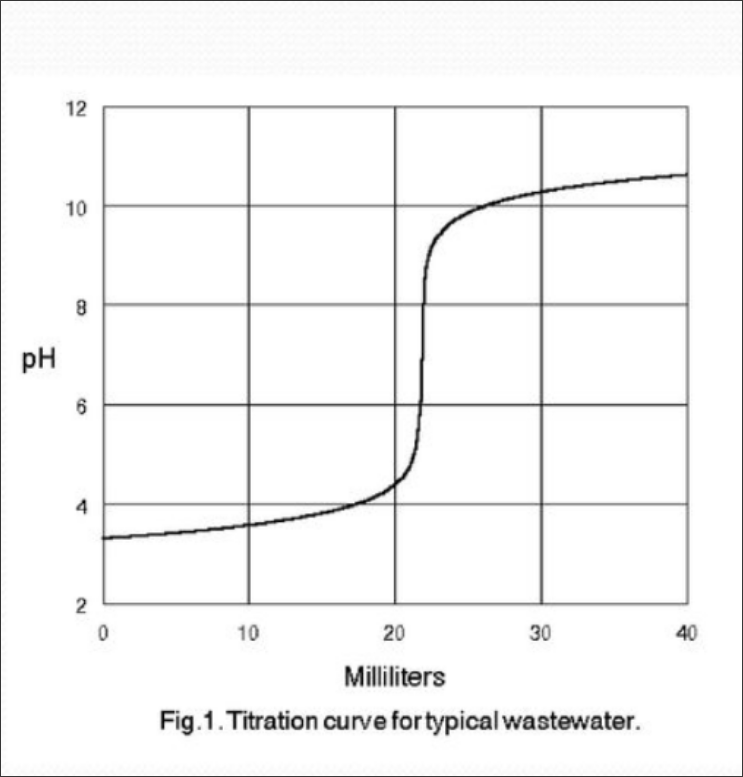
\includegraphics[width=15cm]{ph_curve.png}
		\end{figure}

		When using a pH logger, points beyond the equivalence point should be collected to make the inflexion more obvious

		Polyprotic acids (eg. \ce{H3PO4}) have multiple equivalence points, therefore will have three endpoints. Each "curve" represents the equivalence point of each of the three hydrogen ions

		\begin{figure}[H]
			\centering
			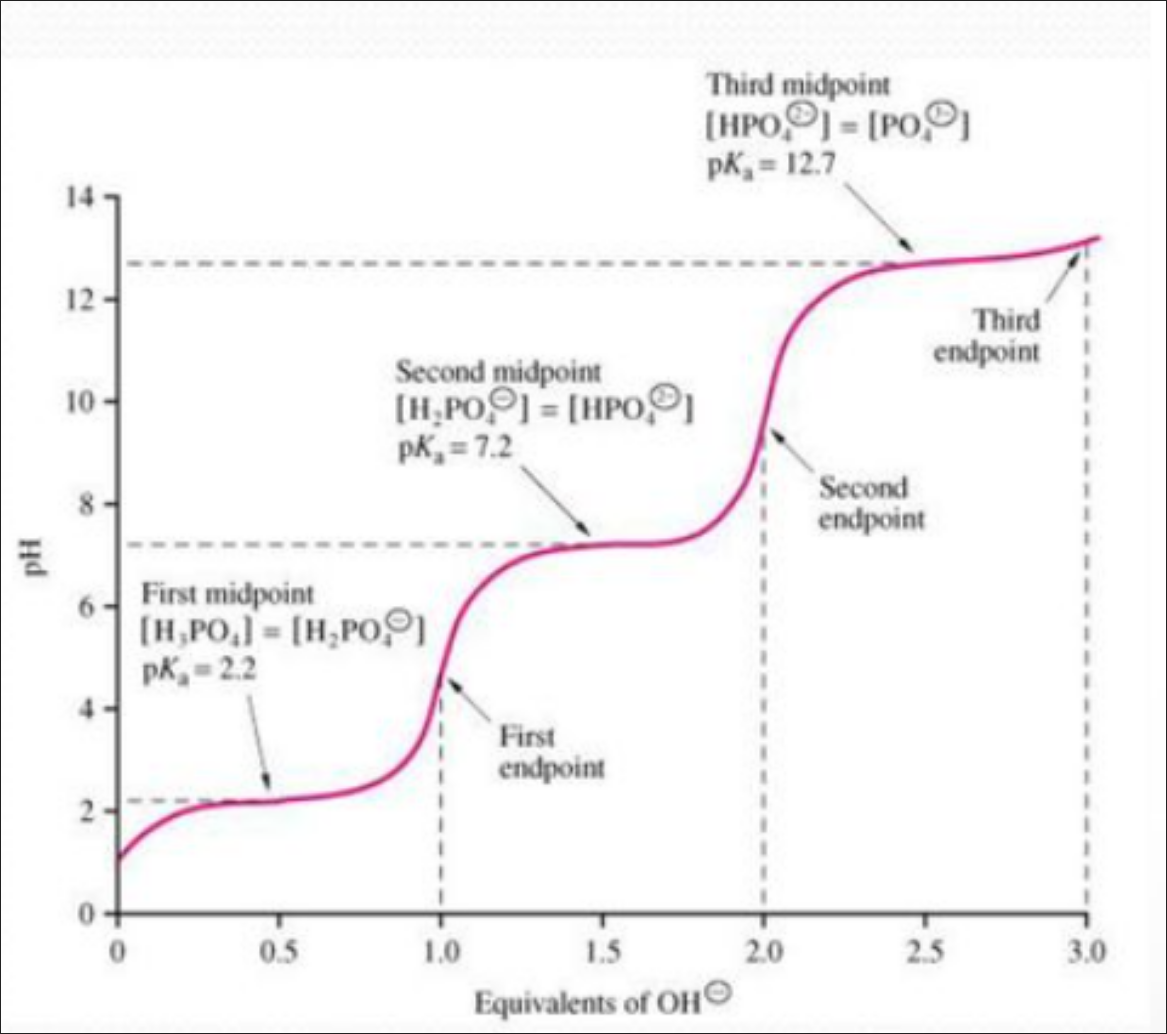
\includegraphics[width=15cm]{polyprotic_curve.png}
		\end{figure}

	\subsection{Activity Sheet 7.4 - Titration Curves}
	
		\subsubsection{Titration of the strong acid in solution}
		
			\begin{enumerate}
				\item What would you expect to be the pH of the titration solution after exact neutralisation of a strong acid with a strong base? If an indicator that changes colour close to this pH were used, would the colour change indicate the equivalence point accurately?
					The pH would be around a pH of 7. If an indicator was used, the pH could be accurately determined through a colour change.

				\item Suppose that we use an indicator that changes colour near pH 5. According to the graph, does the colour change endpoint accurately indicate the equivalence point? Explain why this is the case.

					The equivalence point determined by the graph is around 10. Therefore, an indicator that demonstrates a colour change near a pH of 5 would not be appropriate.

				\item If we use an indicator that changes colour near pH 9, does the colour change endpoint accurately indicate the equivalence point? Explain why.

					Yes. The equivalence point sits around pH 9, therefore an indicator around this would be appropriate.

			\end{enumerate}
		
		\subsubsection{Titration of the weak acid in solution}

			\begin{enumerate}
				\item If a solution of a weak acid is titrated with a NaOH solution, would you expect the pH at exact equivalence to be at pH = 7, at pH $>$ 7, or at pH $<$ 7? Explain why.
					
					\ce{NaOH} is a strong base, therefore when combined with a weak acid the resulting solution would be basic, ie. pH $>$ 7.

				\item Suppose we use an indicator that changes colour near pH 9. Reading the graph as accurately as possible, what volume of titrant (the NaOH solution) is added before the indicator changes colour? Does the indicator colour-change endpoint accurately indicate the equivalence point?
			\end{enumerate}


\section{Acid/base Analysis by Aboriginal and Torres Strait Islander Peoples} \label{20/03/2025}

	\subsection{Grey Mangroves}
	
		The grey mangroves are  used to treat stingray injury by prevent infection and neutralise the mildly acidic stingray venom. This is done by smashing the grey mangroves' leaves to create a basic mixture that can be applied to the wound caused by the stingray

	\subsection{Yellow Ochre}
	
		Aboriginal and Torres Strait Islander Peoples used yell ochre (hydrated iron hydroxide) to treat stomach upsets. The yellow ochre is basic and can react and neutralise with any excess hydrochloric acid in the stomach

	\subsection{Davidson Plum}
	
		The Davidson plum is a natural Australian fruit with 100 times more of ascorbic acid (vitamin C) than contained in an orange. Therefore, it is very sour

		Aboriginal and Torres Strait Islander Peoples consumed the Davidson plum as way to boost their body’s nutrient level which reduced their chance of having scurvy disease.

	\subsection{Soap Tree}
	
		Soap tree's leaves contain saponin acid that has the ability to suppress bateria growth

	\subsection{Goat's Foot (Coastal Morning Glory)}
	
		The leaves (heated on rocks) can be applied as a poultice were used to relieve stings and bites from insects. It is poisonous if incorrectly applied

	\subsection{Clay Eating}
	
		Clay possesses antacid and ati-diarrhoeal functions by assisting with the absorption and assimilation of fluids into the intestine, in which it acts to prevent fluid loss through diarrhoea.

		Clay has the ability to deactivate toxins within the stomach. This increases the tolerance of poisonous plants and unlock a forbidden diet

		It acts as a detoxifying agent. This property is referred to as its poly cationic nature, which leads to the absorption of negative charge toxins. It works like activated charcoal which is known as a digestive aid.

		Its magnetic feature draws cadium, lead, and other toxins to it. The clay moves the toxins molecules through the intestines

\section{Conductometric Titration}

	Another method of determining when the equivalence point is reached is by \textbf{measuring the change in conductivity of the analyte using a conductivity probe}. Conductivity refers to a flow of ions that can be positive or negative, ie. not necessarily electricity. A titration that uses this property is called a conductometric titration.

	\subsection{Advantages}
	
		Can be applied to:
		\begin{itemize}
			\item Very diluted solutions - species at trace levels
			\item Coloured or turbid solutions
			\item Relatively incomplete reactions
			\item Acid-base, redox, precipitation and non-aqueous titrations
		\end{itemize}

	\begin{itemize}
		\item The electrical conductivity of a solution depends on the concentration of ions in the solution
		\item Conductivity of strong base or strong acid is stronger than that of a weak base or weak acid
		\item Change in conductivity during conductometric titration is due to one of the ions being replaced by another of different conductivity
	\end{itemize}

	Equivalence occurs when conductance is at minimum - no free ions. It does not reach 0 because there are still some ions present to transfer charge

	\textbf{Example Question (HSC 2019 Q24)}
	
	The graph initially shows a negative gradient as barium hydroxide solution is introduced into the standardised \ce{HCl} solution. This is due to the reaction of \ce{H+} ions in the \ce{HCl} solution with the \ce{OH-} ions from the barium hydroxide. This decreases the number of conductive ions in the solution, hence decreasing the solution's conductivity. When the equivalence point is reached (around 17mL), the number of \ce{OH-} ions present exceed that of \ce{HCl}, therefore the number of \ce{OH-} ions increases and the graph depicts the solution has an increase in conductivity.

	\textbf{Example Question (HSC 2024 Q34)}
	
	\begin{center}
		\ce{H+(aq) + NH3(aq) -> NH4+(aq)} \\
		\ce{NH3(aq) + HCl(aq) <=> NH4Cl}
	\end{center}

	The graph initially decreases in conductivity as ammonia solution is introduced. This is due to hydrochloric acid being neutralised by the added ammonia.

	The highly conductive \ce{H+} ions react with the \ce{NH3} ions, decreasing the overall conductivity of the solution.

	After the equivalence point, the excess ammonia will produce some \ce{NH4} and \ce{OH-} ions, both of which have greater conductivity than the reactant molecules.

\section{Back Titration} \label{21/03/2025}

	Back titrations are indirect titrations that can be used when:

	\begin{itemize}
		\item the reaction is too slow so it is difficult to determine endpoints
		\item the sample is not soluble in water, but will react with an acid for example
		\item the sample is toxic
		\item the sample is volatile
		\item the sample is gaseous and in a mixture of gases
		\item the sample is fairly unreactive
	\end{itemize}

	\textbf{Example}
	
	A back titration could be used to determine the percentage of calcium carbonate in a sample of limestone. It is not soluble in water, so it cannot be dissolved to form a solution. However, it will react with \ce{HCl}. For example:

	\begin{center}
		\ce{CaCO3(s) + 2HCl(aq) -> CaCl2(aq) + CO2(g) + H2O(l)}
	\end{center}

	A known excess volume of a standardised \ce{HCl} solution (this can be created by titration) would be added to the limestone. It is assumed that the acid only reacts with calcium carbonate, not with any of the other impurities. If the \ce{HCl} reacts with impurities, the final result will be greater than the actual amount of \ce{CaCO3} present.

	The least amount of measurements made reduces the amount of total errors in the experiment and providing a more accurate result.

\section{Titration of Household Chemicals} \label{27/03/2025}

	\subsection{Wine Industry}
		
		The use of analytical instruments in the wine industry allows scientists to learn more about the

		As fermentation proceeds, the density of the mixture decreases. This is due to ethanol's lower density in comparison to water.
	
		Titration to find \ce{SO2} content in wine
		
		Sulphur dioxide is used to kill or inhibit unwanted yeasts and bacteria in wine and to protect the wine from oxidation. When sulphur dioxide is added to wine, there are three forms present: molecular \ce{SO2}, \ce{SO3^{2-}} and smth

	\subsection{Mining Industry}
	
		Ore needs to be dissolved to be tritrated. Done using particular acids. 

\newpage

\section{Buffers} \label{07/04/2025}
	
	\textbf{Keeping the balance}
	
		It is important that environments meet the needs of the organisms that live there. This means that conditions such as pH, concentration of ions, and temperature are maintained at suitable levels.

		In a natural environment, the levels of these conditions in a particular environment will dictate what organisms are able to survive
	
	\subsection{Buffers}
	
		Buffers are utilised in the natural environment and biological systems to maintain an optimal pH.

		It is a solution of a weak acid and its conjugate base (or vice versa) that is \textbf{able to resist a change in pH} when an acid or base is added

		It achieves this due to the equilibrium established between the weak acid (or base) and its conjugate.

		\textbf{Example}
		
		A solution of carbonic acid and sodium hydrogen carbonate (\ce{H2CO3} / \ce{HCO3-})

		The pH of a buffer is determined by the:

		\begin{itemize}
			\item Equilibrium constant $K_a$ of the weak acid
			\item Ratio of weak base [\ce{A-}] to weak acid {\ce{HA}} in solution
		\end{itemize}

		If a buffer has more acid than base, more \ce{H+} ions are present and the pH is lower.

		When the concentrations of \ce{A-} and \ce{HA} are equal, [\ce{H+}] is equal to $K_a$ and the pH is equal to pKa.

		\begin{center}
			\ce{HA(aq) + H2O(l) <=> A-(aq) + H3O+(aq)}
		\end{center}

		When a strong acid is added, LCP pushes the reaction to the left. The pH will increase near to the original value.

		When a strong base is added, the concentration of \ce{H3O} decreases and the system will oppose this change. The pH is decreased to near the original value.

		The pH is maintained by manipulating the proportion of weak base (\ce{A-}) and weak acid (\ce{HA}) in solution. As long as $\frac{[\ce{A-}]}{[\ce{HA}]}$ is between 0.1 and 10, the pH is within 1 unit and the solution is therefore buffered.

	\subsection{Buffer Capacity}
	
		The buffer capacity is the amount of the acid or base that can be added without a significant change in pH. The buffer capacity is greatest when there are equal number of moles of the weak acid and the conjugate base. In this case, it can counteract both the addition of an acid or base. The more of each weak acid and conjugate base, the greater the buffer capacity.

	\subsection{Buffering in the Environment}
	
		With increasing carbon dioxide levels in the atmosphere, there is a major concern that the oceans and soil are being acidified.

		In ocean waters, carbon dioxide is found in higher concentrations than other non-polar gases as it reacts with water. The changes in pH at these levels are significant and are altering the thickness of shells of aquatic organisms and the ability of organisms to take up calcium.

	\subsection{Buffer in sea water}
	
		In sea water, the buffer is due to bicarbonate and carbonate ions.

		In the following reaction:

		\begin{center}
			\ce{HCO3-(aq) + H2O(l) <=> CO3^{2-}(aq) + H3O+(aq)}
		\end{center}

		The \ce{HCO3} is the weak acid, and \ce{CO3^{2-}} is its conjugate base.

		With increasing carbon dioxide levels in the atmosphere, there is a major concern that the oceans are being acidified. The breakdown of organic matter and fish waste also causes the water to become more acidic. The buffer is able to counteract this change so that the pH is not affected.

		Calcium and magnesium ions cause the water to become more alkaline. This happens when items such as shells are added to the environment and when minerals in the surrounding soil are in run-off entering the water.

		Natural sea water has a pH of 8.0 - 8.3. At this pH, there are appropriately equal amounts of bicarbonate and carbonate ions.



\end{document}